\section{Preview of Seiberg-Witten theory} 
We continue our hurried overview from last time.
\subsection{The Seiberg-Witten equations}
Let $(X^4,g)$ be a closed, oriented Riemannian manifold, and let $\mathrm{Sp in}^c(X)$ be the set of isomorphism classes of $\mathrm{sp in}^c$ structures, which acts freely and transitively on $H^2(X;\Z)$. For $\mathfrak s \in  \mathrm{Sp in}^c(X)$, it leads to a spinor bundle $\mathbb S ^{\pm}\to X$, which is a rank 2 and hermitian vector bundle. Clifford mulitplication is given by $T^*X \xrightarrow{\rho} \Hom(\mathbb S^+, \mathbb S^-)$, and the configuration space $\mathcal C = \{ \text{spin connections } \nabla \text{ in } \mathbb S^+\} \times  \Gamma (X,\mathbb S^+)$ where $\Gamma(X,\mathbb S^+)$ consists of $C ^{\infty}$ sections of $\mathbb S^+$. The set of spin connections is identified with $U(1)$ connections in $\det \mathbb S^+ = \Lambda^2 \mathbb S^+ $. The gauge group is given by $\mathcal G= C^{\infty}(X, U(1))$, and define $\mathcal B = \mathcal C / \mathcal G$.  A $\mathcal G$-action on $\mathcal C$ is free except at ``irreducible configurations'', $(\nabla,0) \in \Gamma(\mathbb S^+)$. The set of irreducible configurations $\mathcal C^* \to \mathcal B^* = \mathcal C^* / \mathcal G$ which has the same homotopy type of $\mathcal P = \frac{H^1(X,\R)}{H^1(X,\Z)}\times \C \mathrm{P }^{\infty}$, $\Gamma(\mathbb S^+) / U(1)$. Then 
\begin{align*}
    H_*B^* &= H_*(\mathcal P \times \C \mathrm{P}^{\infty})\\
           &= H_*\mathcal P \otimes H_* (\C \mathrm{P}^{\infty}) \quad \text{(plus torsion terms)} \\
           &= \Lambda^* H^1(X;\Z) \otimes \Z[U] \quad \text{(deg 2)} 
\end{align*}
There were then the Seiberg-Witten equations; for a pair $(\nabla,\phi)$, this induces a connection $\nabla^t $ in $\Lambda^2\mathbb S^+$, and therefore is a configuration in $\mathcal C$. The equations are as follows:
\begin{itemize}
\setlength\itemsep{-.2em}
    \item \textbf{Dirac equation:} $D_{\nabla}\phi = 0$, where $D$ is the \emph{Dirac operator} (a linear first order differential operator taking sections $\Gamma(\mathbb S^+) \to \Gamma(\mathbb S^-)$). This is an affine bilinear equation in $(\nabla,\phi)$.
    \item \textbf{Curvature equation:} The Clifford equation $\rho$ induces an endomorphism $\rho \colon \Lambda^+ \to \mathfrak{su}  (\mathbb S^+)$. Then apply $\rho $ to get $\rho(F_{\nabla^t} = (\phi \otimes \phi^*)_0$ (the subscript 0 means trace free).
    \item We also impose a Coulomb gauge fix on $\nabla^t$, where $d^*(\nabla^t - \nabla^t _{\mathrm{ref}}) = 0$. 
\end{itemize}
These three equations together are \textbf{elliptic}. That implies that their linearization at a solution is \textbf{Fredholm}, which is to say it has finite dimensional kernel and cokernel. 

There are the reducible solutions, where $(\nabla,\phi)\phi\equiv 0$. The Dirac equation becomes vacuous, and $Fs_{\nabla^t}^+ = 0$, i.e., $\nabla^t$ is an \emph{instanton} in $\det \mathbb S^+$. If $b^+ > 0$ and $\det \mathbb S^+$ is a non-trivial line bundle, then there do not exist instantons for generic conformal structures $g$ (proved in class modulo the proof of the Hodge theorem). Then all solutions to the Seiberg-Witten equations are \emph{irreducible}. So we have the \textbf{Seiberg-Witten moduli space} $\mathcal M _{\mathfrak s, g}\subseteq \mathcal B^*$. The nice situation is when the linearization of the SW equations at any solution is surjective, or $\coker = 0$. This is the the transverse case, and in this case, $\mathcal M _{\mathfrak s, g}$ is a submanifold of $\mathcal B^*$. In general, one proves a generic transversality theorem; for generic metrics $g$, the nice situation applies. The dimension of the moduli space is given by \[
    \dim \mathcal M_{\mathfrak g, g}= \dim \ker \mathcal D_{(\nabla,\phi)} = \operatorname{index}\mathcal D_{(\nabla,f)} = \frac{1}{4}\left( c_1(\Lambda^2 \mathbb S^+) ^2[X] - 2\chi(X) - 3 \tau(X) \right)  \in \Z
\]where $\mathcal D$ is the linearization of SW, and the index is $\dim \ker - \dim \coker$. The index is much better behaved, and can be computed by topological formulas like the Atiyah-Singer index theorem, which leads to the formulation above. Here $c_1(\Lambda^2\mathbb S^+)$ is the characteristic vector. Then a Seiberg-Witten miracle happens; $\mathcal M _{\mathfrak s, g}$ is compact. Towards the end of the course we talk about the proof of this fact. It is also orientable; an orientation for $H^0 _{\mathrm{DR}}(X) \oplus H^1_{\mathrm{DR}}(X) \oplus \mathcal H^+_{\mathcal G}(X)$ determines an orientation for $\mathcal M _{\mathfrak s,g}$ (we call this a ``homology orientation''). Then we have a fundamental homology class $[\mathcal M_{\mathfrak s, g}] \in H_{d(\mathfrak s)}(\mathcal B^*)$, and $\mathrm{SW}_X(\mathfrak s)$ is essentially $[\mathcal M_{\mathfrak s,g}] \in  (\Lambda^* H^1\otimes \Z[U])$. In many cases $d(\mathfrak s) = 0$, and $\mathcal M _{\mathfrak s, g}$ is an oriented 0-manifold, or a signed set of points. Then $\mathrm{SW}_X(\mathfrak s) = \# \mathcal M_{\mathfrak s, g}$.

What justifies calling this a Seiberg-Witten \emph{invariant}? We have a parameter here, the metric. So we need to check metric invariance. Consider $\mathcal M_{\mathfrak s, g_0}$ versus $\mathcal M_{\mathfrak s,g_1}$. Pick a generic path $\{g_t\} $ of metrics. Then the parametric moduli space is given by $\mathcal D = \{(t \in [0,1], [\nabla,\phi] \in \mathcal M _{\mathfrak s, g_t}\} $. This gives a cobordism from $\mathcal M _{\mathfrak s, g_0} \to \mathcal M _{\mathfrak s, g_1}$; 
\begin{figure}[H]
\centering
 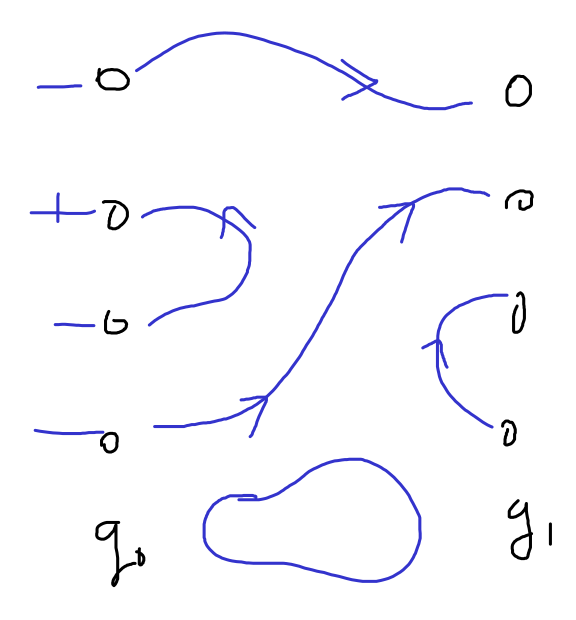
\includegraphics[width=0.3\linewidth]{figures/cobord.png}
\caption{The cobordism of moduli spaces.}
\label{cobord}
\end{figure}
We need $\mathcal P$ cut out transversely insides $[0,1] \times \mathcal B^*$, avoiding reducible solutions for all $g_t$. If  $b^+ > 1$, generic paths of metrics have no instantons. If $b^+  = 1$, we could encounter instantons in the path. This is the outcome:
\begin{itemize}
\setlength\itemsep{-.2em}
    \item If $b^+ X> 1$, we get $\mathrm{SW}_X \colon  \mathrm{Sp in}^c (X) \to \Z$, and  
        \[
        \mathrm{SW}_X(\mathfrak s) = 
        \begin{cases}
            \langle [\mathcal M_{\mathfrak s,g}], U ^{d(\mathfrak (s) / 2} \rangle & \text{if } d(\mathfrak s ) \in 2\Z,\\
            0 & \text{if } d(\mathfrak s) \text{ is odd.} 
        \end{cases}
        \] 
    \item If $b^+ X = 1$, $\mathrm{SW_X}$ depends on additional data.
    \item If $b^+X = 0$, we have no meaningful invariant.
\end{itemize}
We still need to talk about spin geometry and elliptic operators. Then we will get into Seiberg-Witten specific things like the compactness of the moduli space.


